\documentclass{beamer}
%%%%%%%%%%%%%%%%%%%%%%%%%%%%%%%  Packages  %%%%%%%%%%%%%
\usepackage{amsmath} 
\usepackage{mathtools}
\usepackage{physics}
\usepackage{amssymb}
\usepackage{mathptmx}
\usepackage{array}
  
%%%%%%%%% FIGurES %%%%%%%%%%%%%%%%%%%%%%%%
\usepackage{textcomp}
\usepackage{graphicx}
\usepackage{caption} 
\usepackage{subcaption}
\usepackage{scrextend}
\usepackage{rotating}
\usepackage{float}
\usepackage{hyperref}

\graphicspath{{./figures/}}
\hypersetup{colorlinks=true, citecolor=blue, linkcolor=blue}
\renewcommand{\equationautorefname}{Eq.}
\renewcommand{\figureautorefname}{Fig.}
 
%%%%%%%%%%%% LaNgUaGe %%%%%%%%%%%%%%%%%%
\usepackage{verbatim}
\usepackage{natbib}
%\usepackage{qcircuit}
\usepackage{wrapfig}

\usepackage{minted}

\usepackage[utf8]{inputenc}
\usetheme{PaloAlto}

\setminted[bash]{breaklines}

\title{Version control using Git and Plotting Tutorial}
\author{Oliver Thomas}
\institute{Quantum Engineering CDT \\ University of Bristol}
\date{\today}

% plan


\begin{document}

\frame{\titlepage}



\begin{frame}{Overview}


\begin{itemize}
        \item Version control
        \item Plotting using gnuplot
        \item Vim
    \end{itemize}
\end{frame}

% slide 1
\begin{frame}
\frametitle{Why you should use version control}
\begin{itemize}
	\item Does this seem familiar? 
\end{itemize}

\begin{figure}[H]
	\centering
	
\includegraphics[width=0.26\textwidth]{xkcdversion.png}
	\caption{Bad version control\footnote{\url{https://xkcd.com/1459/}}}
	\label{fig:xkcdversion}
\end{figure}
\end{frame}

%slide 2
\begin{frame}
\frametitle{What is Git?}
\begin{itemize}
\item Git is one of most used version control software in the world 
\item Git is cross-platform and easy to use \footnote{\url{https://try.github.io/levels/1/challenges/1}}
\end{itemize}
\end{frame}

%slide 2
\begin{frame}
\frametitle{What is GitHub?}
\begin{itemize} 
\item Github is a cloud service for git which lets you store your repository online
\item Why would you store your repository online?
\begin{itemize}
\item Working remotely
\item Collaborative work  
\item Hard drive failure!
\end{itemize}
\end{itemize}
\end{frame}


%slide 3
\begin{frame}
\frametitle{Making a repository}
\begin{itemize}
\item You can do this online on the Github website \footnote{\url{https://github.com/}}
\item Create a new repository
\item Then click clone to get the url, open git on your computer and type: \\ 
	\texttt{git clone url}
\end{itemize}
\end{frame}

%slide 3
\begin{frame}
\frametitle{Making a repository}
\begin{itemize}
	\item Go to the folder and right click \texttt{git with bash}
\item You are now able to use bash for the rest of the talk!
\end{itemize}
\end{frame}

%slide 4
\begin{frame}
\frametitle{Basic Git commands}
\begin{itemize}
	\item There are four\footnote{I cheat here and write a bash script which does these in order so I only have to run a single command.} important commands you will need for git:
	\item \texttt{git pull}
	\item \texttt{git add *}
	\item \texttt{git commit -a}
	\item \texttt{git push}
\end{itemize}
\end{frame}


% slide editors
\begin{frame}{A brief note on text editors: Vim}
    \begin{itemize}
    \item Vim is a powerful cross-platform text editor, released in 1991 and is still regarded as one of the most popular editors \footnote{Along with Emacs}. 
    \item Flexible with thousands of plugins available e.g. I use Vim to compile latex documents, this presentation was written in Vim.  
    \item Computing clusters normally only have CLI so if you are running high performance code you will need to be familiar with Vim, Emacs or Nano.
    \item You can feel like a Hacker.
\end{itemize}
\end{frame}

\begin{frame}{Vim commands}
    \begin{itemize}
        \item The most important thing to remember is that Vim has two main modes, \textit{NORMAL}, \texttt{ESC} and \textit{INSERT}, \texttt{i}
        \item All commands are run from \textit{NORMAL} mode using \texttt{:}
        \item to quit use, \texttt{ESC:q} (meaning go to \textit{NORMAL} mode, \texttt{:} means command and \texttt{q} is quit without saving)
        \item to save and quit use, \texttt{ESC:wq} (\texttt{w} stands for write)
    \end{itemize}

\end{frame}

%slide 2
\begin{frame}
	\frametitle{Adding your first commit}
\begin{itemize}
    \item Every repository should contain a readme
	\item Then either run: 
	\item \texttt{git add *}
	\item \texttt{git commit -a}
	\item \texttt{git push}
\end{itemize}

Or use the windows GUI version and commit them to your repository.
\end{frame}

%slide 5
\begin{frame}
\frametitle{gnuplot} 
\begin{itemize}
	\item Gnuplot is popular, multi-platform and standard software on computing clusters\footnote{standard on most of the popular linux distributions} 
    \item \url{https://sourceforge.net/projects/gnuplot/files/gnuplot/5.2.4}
\end{itemize}
\end{frame}

%%%%%%%%%%%%%%%%%%%%%%%%%%%%%%%%%%%%%%%%%%%%%%%%%%%%%%%%%%%%%%%%%
%slide gnuplot 1
\begin{frame}[fragile]
    \frametitle{Example 0 Quick plotting}
\begin{itemize}
	\item Go to the \texttt{src} folder
    \item open gnuplot and type \\ \texttt{plot 'data.txt'}
\end{itemize}
\end{frame}

%slide 2
\begin{frame}{Example 0 Quick plotting}
    \begin{figure}
	\centering
	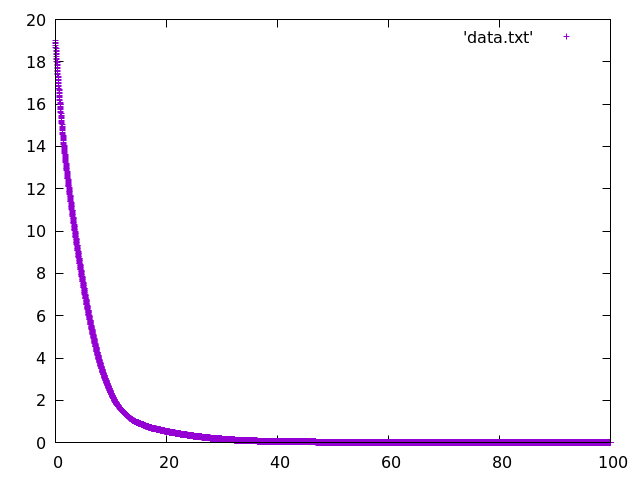
\includegraphics[width=0.6\textwidth]{src/data.png}
	\caption{function plotting}
	\label{fig:function}
\end{figure}
Lets you very quickly see what the data is doing
\end{frame}

%%%%%%%%%%%%%%%%%%%%%%%%%%%%%%%%%%%%%%%%%%%%%%%%%%%%%%%%%%%%%%
%slide gnuplot 1
\begin{frame}[fragile]
    \frametitle{Example 1 Plotting functions}
\begin{itemize}
	\item Go to the \texttt{src} folder
    \item open gnuplot and type \\ \texttt{load 'ex1\_basic.p'}
\end{itemize}
\inputminted{bash}{src/ex1_basic.p}
\end{frame}

%slide saving plots gnuplot 
\begin{frame}[fragile]
    \frametitle{Example 2 Saving plots}
\begin{itemize}
	\item Go to the \texttt{src} folder
    \item open gnuplot and type \\ \texttt{load 'ex2\_saving.p'}
\end{itemize}
\inputminted{bash}{src/ex2_saving.p}
\end{frame}

%slide 2
\begin{frame}{Example 2 Plotting functions}
    \begin{figure}
	\centering
	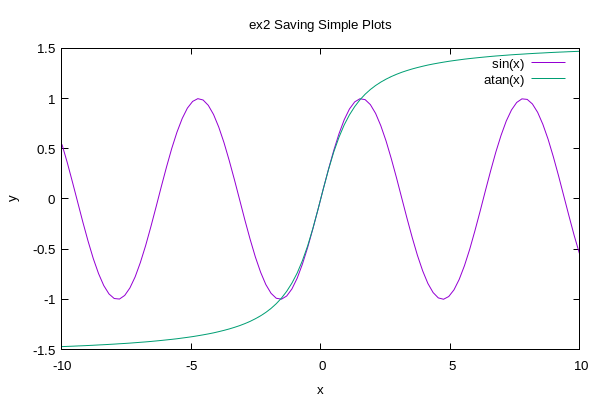
\includegraphics[width=0.6\textwidth]{src/ex2.png}
	\caption{function plotting}
	\label{fig:function}
\end{figure}
Produces a png
\end{frame}

%%%%%%%%%%%%%%%%%%%%%%%%%%%%%%%%%%%%%%%%%%%%%%%%%%%%%%%%%%%%%%%%
%slide 2
\begin{frame}
\frametitle{Example 3 Plotting data!}
\begin{itemize}
	\item once again, in the \texttt{src} folder open \texttt{ex3data.py}
	\item Run all.py and choose 3 
\end{itemize}
\end{frame}

%slide 2
\begin{frame}
\frametitle{Example 3 Plotting data!}
\begin{itemize}
	\item figure 
\end{itemize}
\begin{figure}
	\centering
	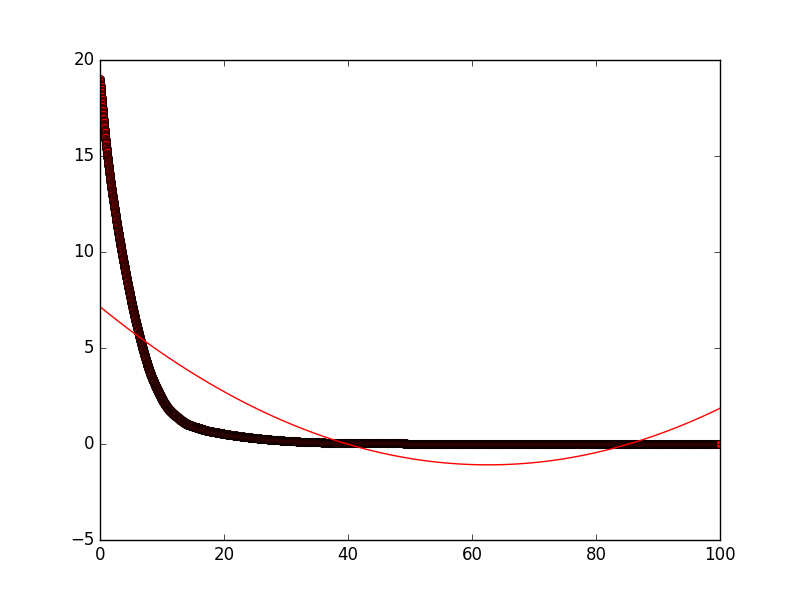
\includegraphics[width=0.5\textwidth]{ex3.png}
	\caption{function plotting}
	\label{fig:function}
\end{figure}
\end{frame}



%%%%%%%%%%%%%%%%%%%%%%%%%%%%%%%%%%%%%%%%%%%%%%%%%%%%%%%%%%%%%%%%
%slide subplots
\begin{frame}
\frametitle{Example 5, Subplots!}
\begin{itemize}
\item In the \texttt{src} folder open \texttt{ex5subplots.py} 
	\item Run all.py and choose 5 
\end{itemize}
\end{frame}

%slide 2
\begin{frame}
\frametitle{Example 5, Subplots!}
\begin{itemize}
\item Figures!
\end{itemize}
\begin{figure}
	\centering
	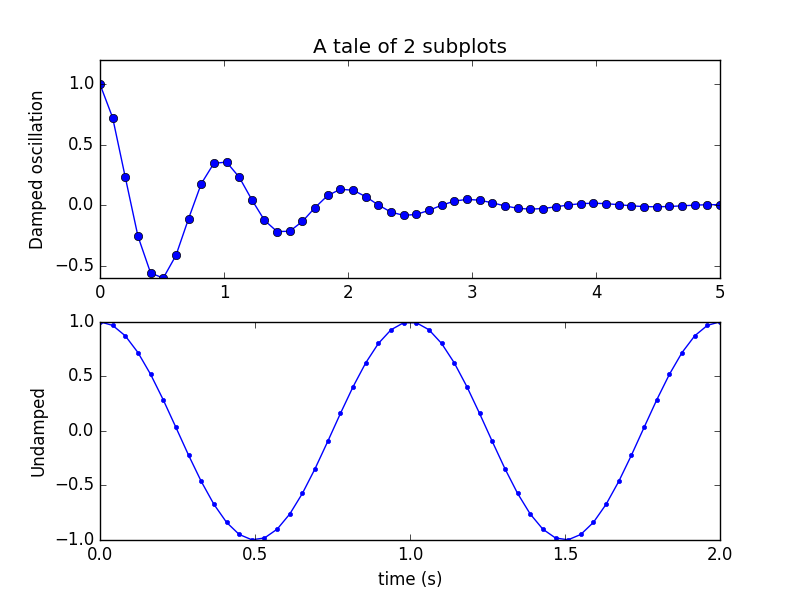
\includegraphics[width=0.5\textwidth]{ex5.png}
	\caption{function plotting}
	\label{fig:function}
\end{figure}
\end{frame}


%%%%%%%%%%%%%%%%%%%%%%%%%%%%%%%%%%%%%%%%%%%%%%%%%%%%%%%%%%%%%%%%
%slide 2
\begin{frame}
\frametitle{Example 4, Histograms!}
\begin{itemize}
\item once again, in the \texttt{src} folder open \texttt{ex4hist.py}
	\item Run all.py and choose 4 
\end{itemize}
\end{frame}

%slide 2
\begin{frame}
\frametitle{Example 4, Histograms!}
\begin{itemize}
\item figure
\end{itemize}
\begin{figure}
	\centering
	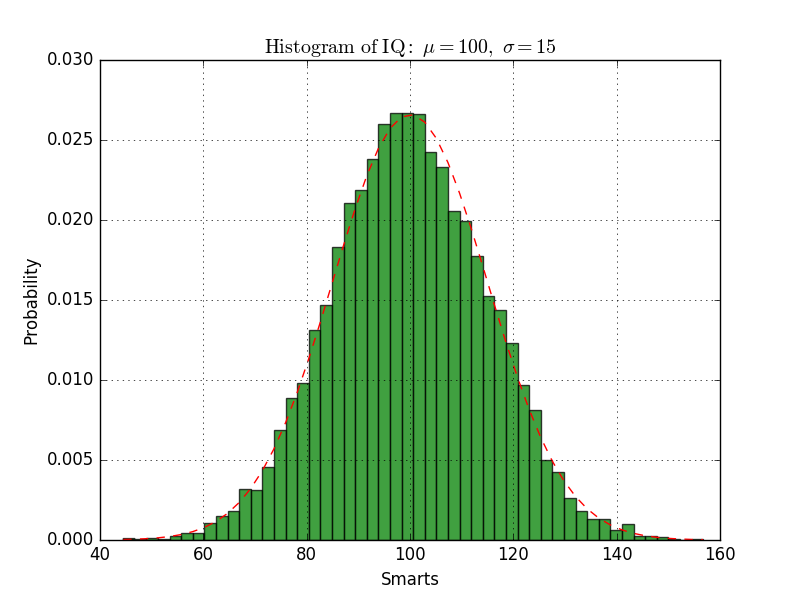
\includegraphics[width=0.5\textwidth]{ex4.png}
	\caption{function plotting}
	\label{fig:function}
\end{figure}
\end{frame}

%%%%%%%%%%%%%%%%%%%%%%%%%%%%%%%%%%%%%%%%%%%%%%%%%%%%%%%%%%%%%%%%
%slide 4
\begin{frame}
\frametitle{Advanced Git commands}
\begin{itemize}
    \item One of the great things about Git is that you can get by with just the four (main) commands mentioned earlier.
	\item The git man page is very useful, especially, \\
	\texttt{man gittutorial} \\
	\texttt{man giteveryday} \\ 
\item \texttt{giteveryday} is a super useful collection of the 20 commands you will need regularly.
\end{itemize}
\end{frame}


%slide 2
\begin{frame}
\frametitle{Branching}
\begin{itemize}
\item Branching is useful, it lets you test something out separately to the main branch.
\item To make a new branch called \texttt{test} \\
\texttt{git branch test} 
\item You can check all of the current branches and which branch you are on with \\
	\texttt{git branch}
\end{itemize}
\end{frame}

%slide 2
\begin{frame}
\frametitle{Branching}
\begin{itemize}
	\item To switch to the test branch type: \\ 
	\texttt{git checkout test} \\
\end{itemize}
\end{frame}

%slide 4
\begin{frame}
\frametitle{Adding Collaborators}
\begin{itemize}
	\item Go to a repository and on the settings tab click collaborators, you can then search for the github username
\end{itemize}
\end{frame}


%slide 2
\begin{frame}
\frametitle{Thanks for listening!}
\begin{figure}[H]
	\centering
	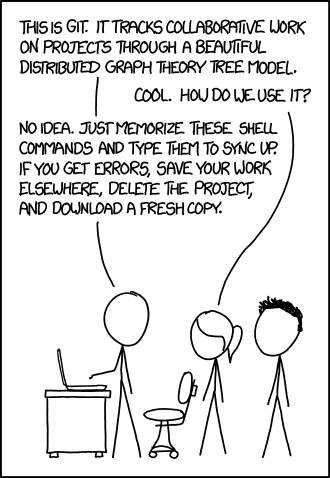
\includegraphics[width=0.4\textwidth]{xkcdgit.png}
	\caption{If it all goes wrong \ldots \footnotemark }
	\label{fig:xkcdversion}
\end{figure}
\footnotetext[1]{\url{https://xkcd.com/1597/}}
\end{frame}


\end{document}
